% Created 2017-03-11 sam. 11:55
% Intended LaTeX compiler: pdflatex
\documentclass[bigger]{beamer}
\usepackage[utf8]{inputenc}
\usepackage[T1]{fontenc}
\usepackage{graphicx}
\usepackage{grffile}
\usepackage{longtable}
\usepackage{wrapfig}
\usepackage{rotating}
\usepackage[normalem]{ulem}
\usepackage{amsmath}
\usepackage{textcomp}
\usepackage{amssymb}
\usepackage{capt-of}
\usepackage{hyperref}
\usetheme{Boadilla}
\author{Christophe Goudet}
\date{\today}
\title{ROOT/RooFit fit difference}
\beamertemplatenavigationsymbolsempty
\usepackage{appendixnumberbeamer}
\hypersetup{
 pdfauthor={Christophe Goudet},
 pdftitle={ROOT/RooFit fit difference},
 pdfkeywords={},
 pdfsubject={},
 pdfcreator={Emacs 24.5.1 (Org mode 9.0.4)},
 pdflang={English}}
\begin{document}

\maketitle

\section{Introduction}
\label{sec:org292386b}
\begin{frame}[label={sec:org5d0baf9}]{Introduction}
\begin{itemize}
\item Marc observed a difference in fit results depending on using ROOT or RooFit
\begin{itemize}
\item "looks like" RooFit does not consider uncertainties in weighted RooDataHist
\end{itemize}
\item Checked if effect has visible effects on calibration systematic determination for couplings analysis.
\item 4 fit methods compared :
\begin{itemize}
\item nominal : fit of weighted binned RooDataHist
\item unbinned : fit of weighted unbinned RooDataSet
\item root : fit of weighted binned TH1
\item meanHist : mean and RMS of weighted binned TH1
\end{itemize}
\end{itemize}
\end{frame}

\begin{frame}[label={sec:org164a9b8}]{Inclusive Fit Values}
\begin{center}
\tiny
\begin{tabular}{lrrrrrr}
\hline
NP & mean & sigma & alphaHi & alphaLow & nHi & nLow\\
\hline
\hline
RooFit &  &  &  &  &  & \\
\hline
Nominal & 125.026 & 1.80019 & 1.40272 & 1.27818 & 42.7717 & 10.9658\\
EG-RESOLUTION-ALL--1down & 125.029 & 1.67024 & 1.40272 & 1.27818 & 42.7717 & 10.9658\\
EG-RESOLUTION-ALL--1up & 125.022 & 1.93601 & 1.40272 & 1.27818 & 42.7717 & 10.9658\\
EG-SCALE-ALL--1up & 125.59 & 1.83223 & 1.40272 & 1.27818 & 42.7717 & 10.9658\\
EG-SCALE-ALL--1down & 124.46 & 1.80542 & 1.40272 & 1.27818 & 42.7717 & 10.9658\\
\hline
\hline
Root &  &  &  &  &  & \\
\hline
Nominal & 125.032 & 1.84212 & 1.6817 & 1.37856 & 6.73971 & 7.27819\\
EG-RESOLUTION-ALL--1down & 125.033 & 1.70918 & 1.6817 & 1.37856 & 6.73971 & 7.27819\\
EG-RESOLUTION-ALL--1up & 125.03 & 1.97901 & 1.6817 & 1.37856 & 6.73971 & 7.27819\\
EG-SCALE-ALL--1down & 124.464 & 1.8484 & 1.6817 & 1.37856 & 6.73971 & 7.27819\\
EG-SCALE-ALL--1up & 125.598 & 1.87389 & 1.6817 & 1.37856 & 6.73971 & 7.27819\\
\hline
\end{tabular}
\end{center}
\end{frame}
\begin{frame}[label={sec:org1da5e7c}]{Inclusive results in ALL model}
\begin{itemize}
\item Binned or unbinned fit with RooFit give similar results
\item RooFit or Root give sligthly different systematics
\end{itemize}

\begin{columns}
\begin{column}{0.5\columnwidth}
\begin{center}
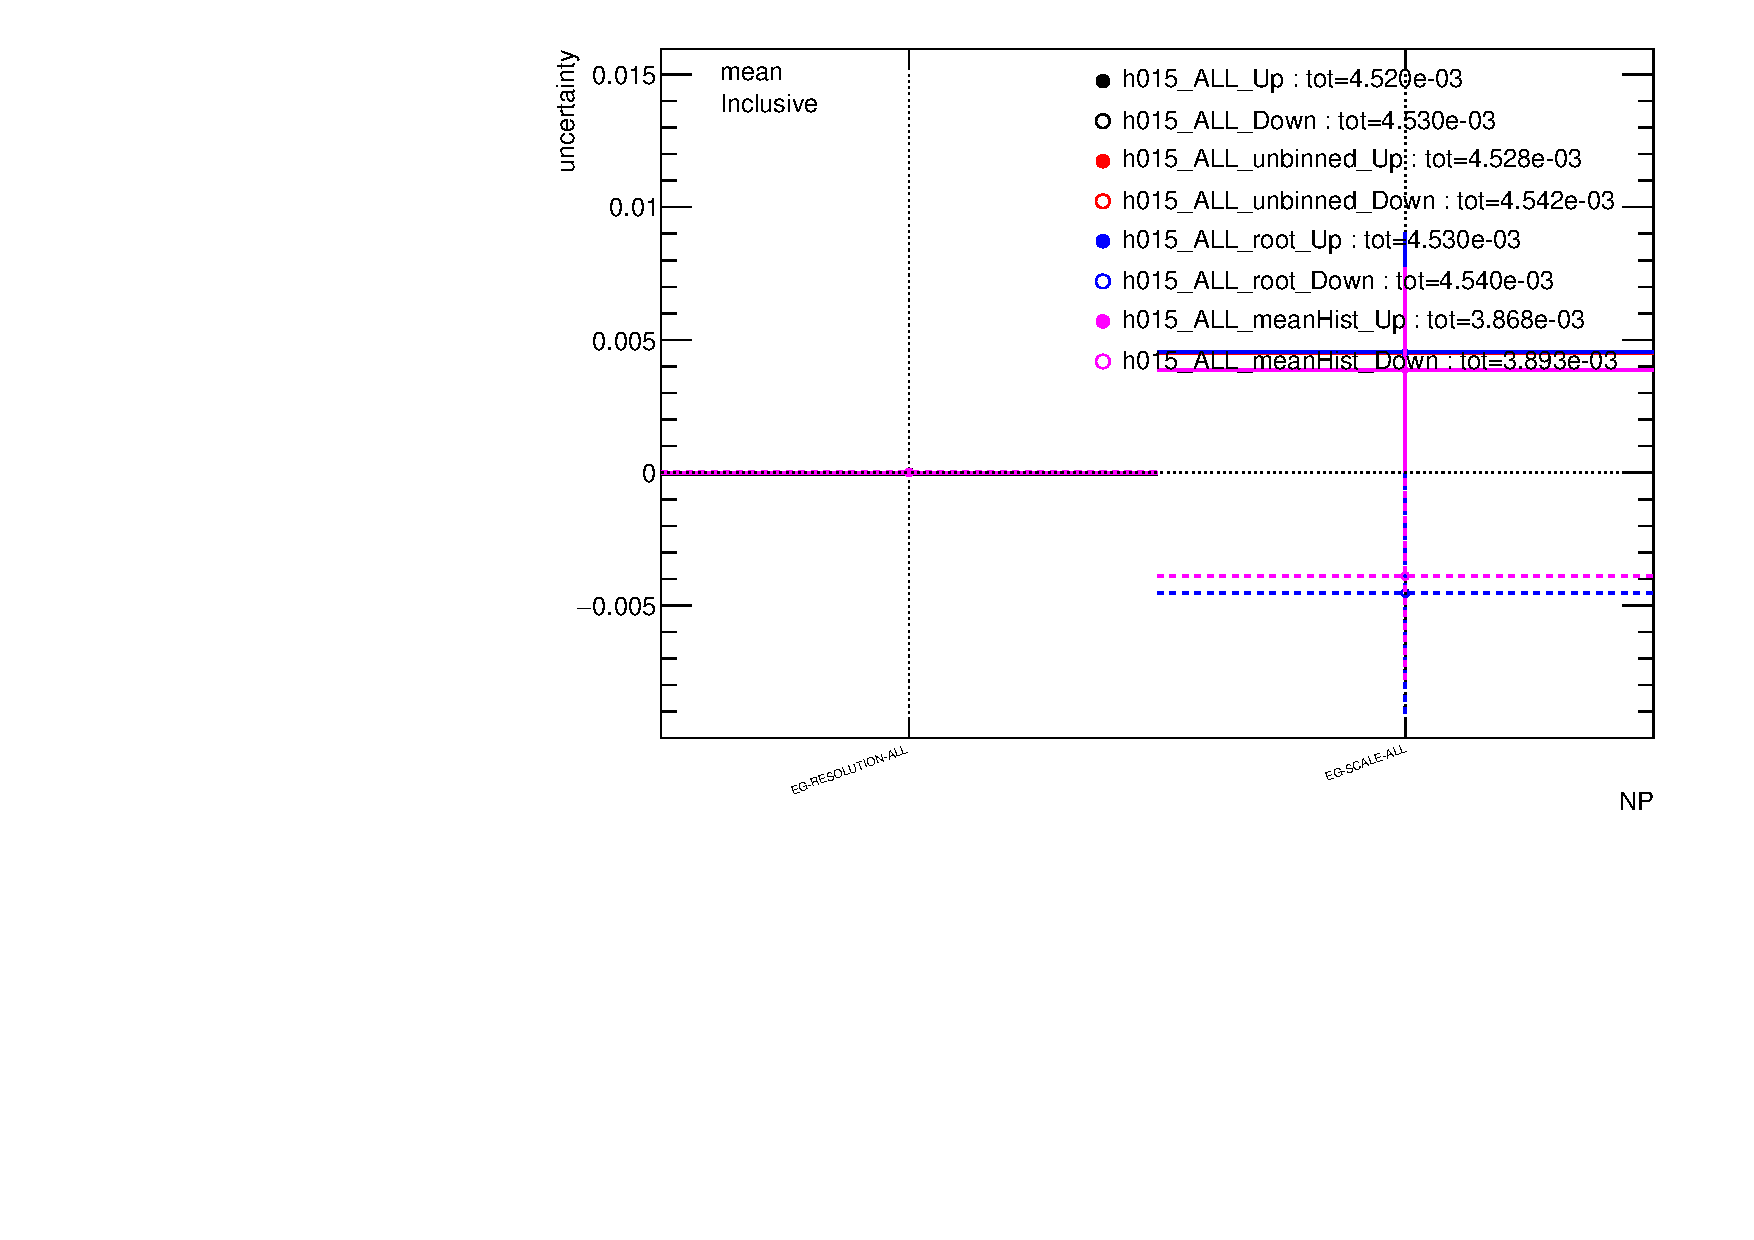
\includegraphics[width=.9\linewidth]{/home/goudet/Documents/LAL/Slides/Misc/plots/CompareFits_Systematics_Inclusive_mean_mean.pdf}
\end{center}
\end{column}

\begin{column}{0.5\columnwidth}
\begin{center}
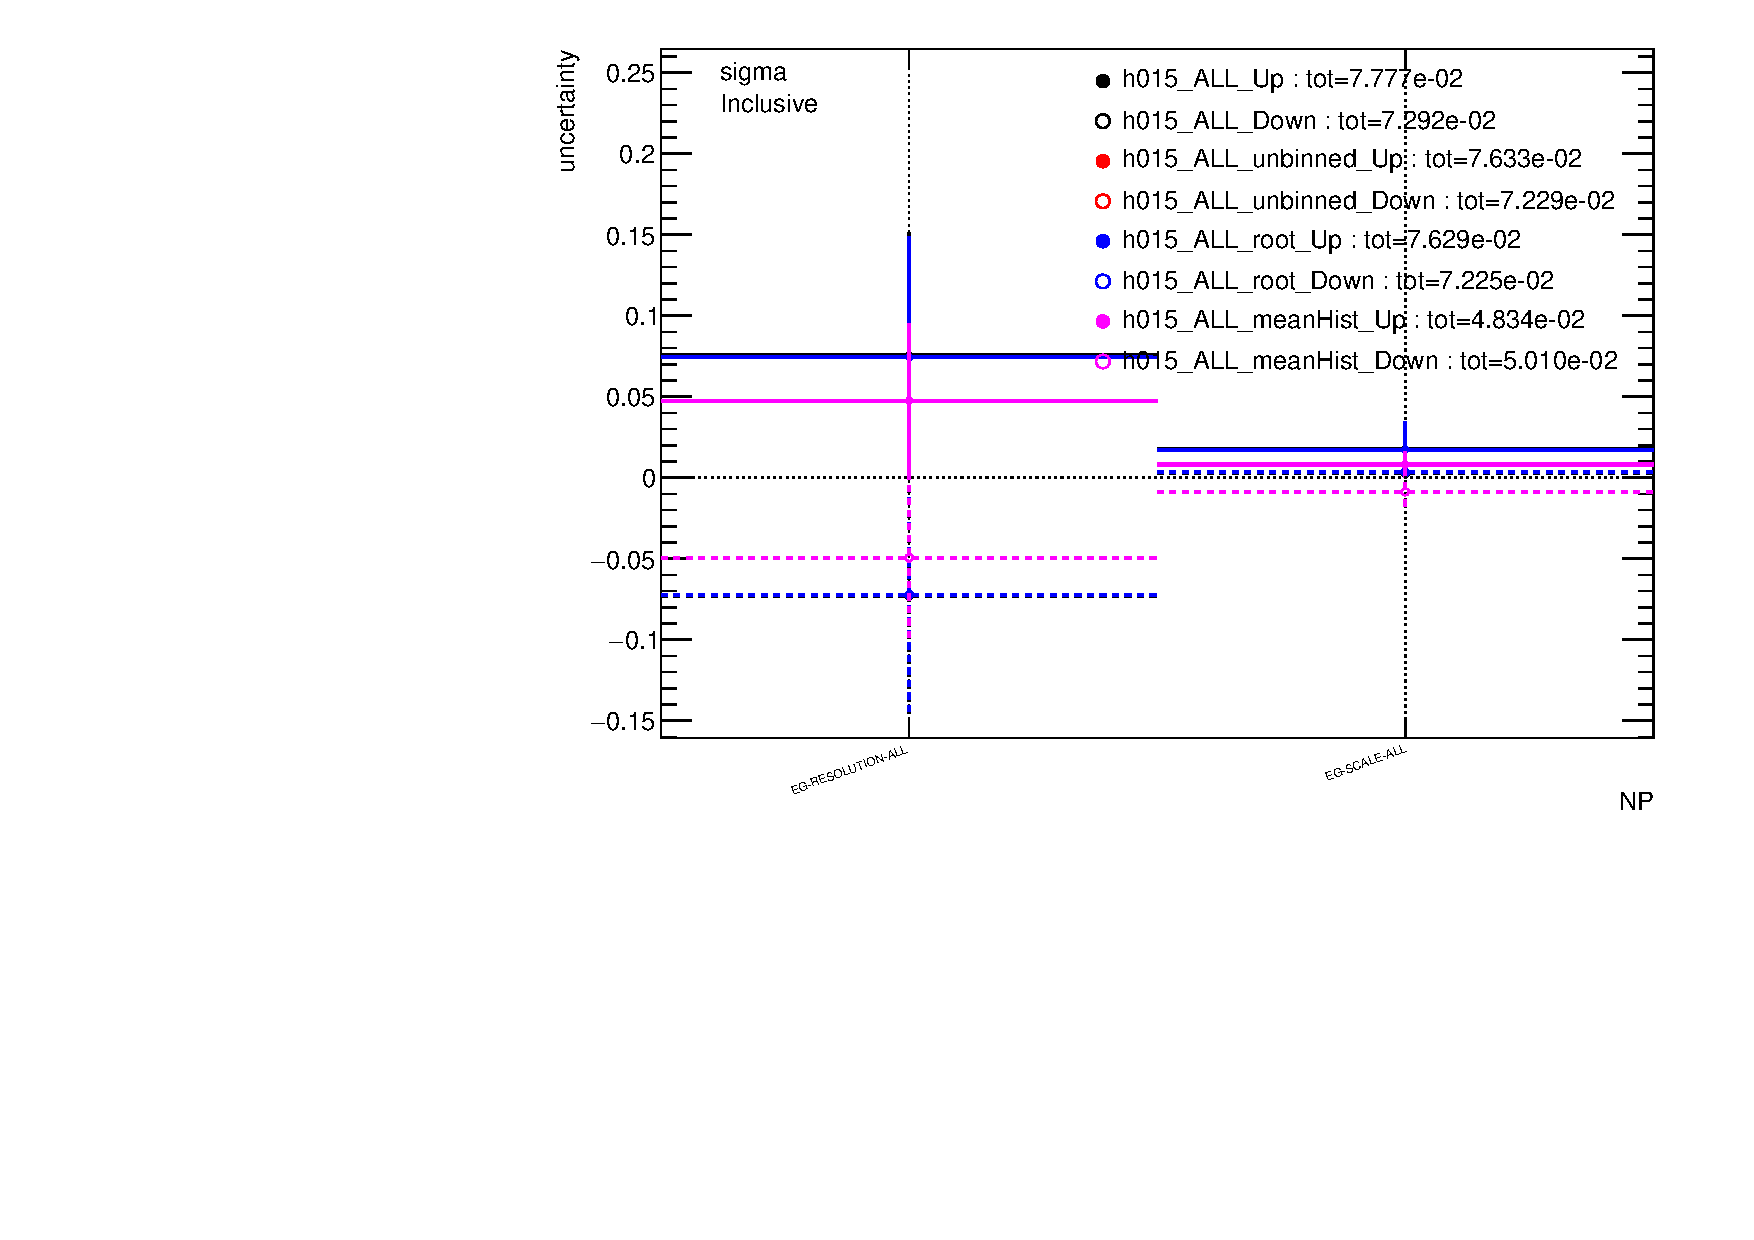
\includegraphics[width=.9\linewidth]{/home/goudet/Documents/LAL/Slides/Misc/plots/CompareFits_Systematics_Inclusive_sigma_sigma.pdf}
\end{center}
\end{column}
\end{columns}
\end{frame}
\begin{frame}[label={sec:orgb852827}]{Fits}
\begin{columns}
\begin{column}{0.45\columnwidth}
\begin{center}RooFit\end{center}
\begin{center}
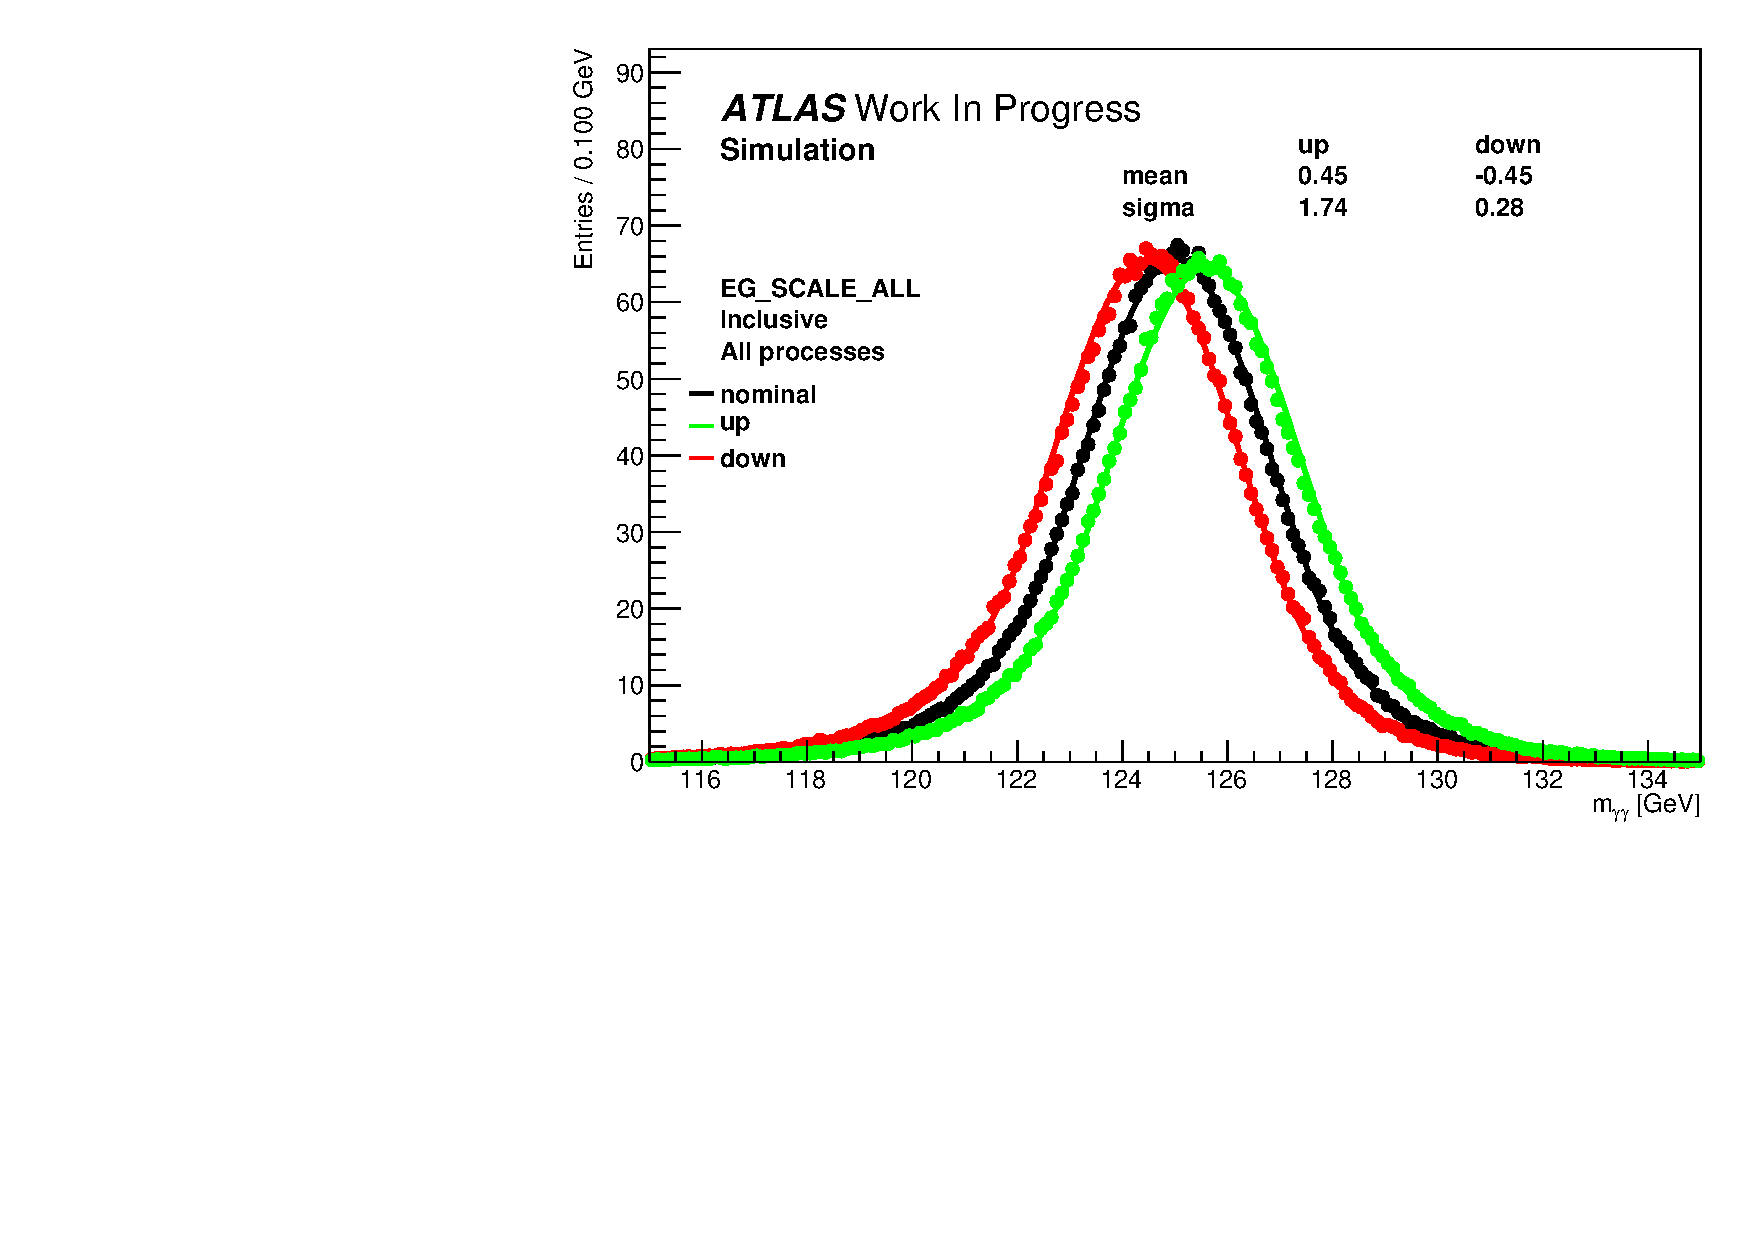
\includegraphics[width=.9\linewidth]{/home/goudet/Documents/LAL/Slides/Misc/plots/h015_ALL_SystVariation_EG_SCALE_ALL_0.pdf}
\end{center}
\end{column}

\begin{column}{0.45\columnwidth}
\begin{center}ROOT\end{center}
\begin{center}
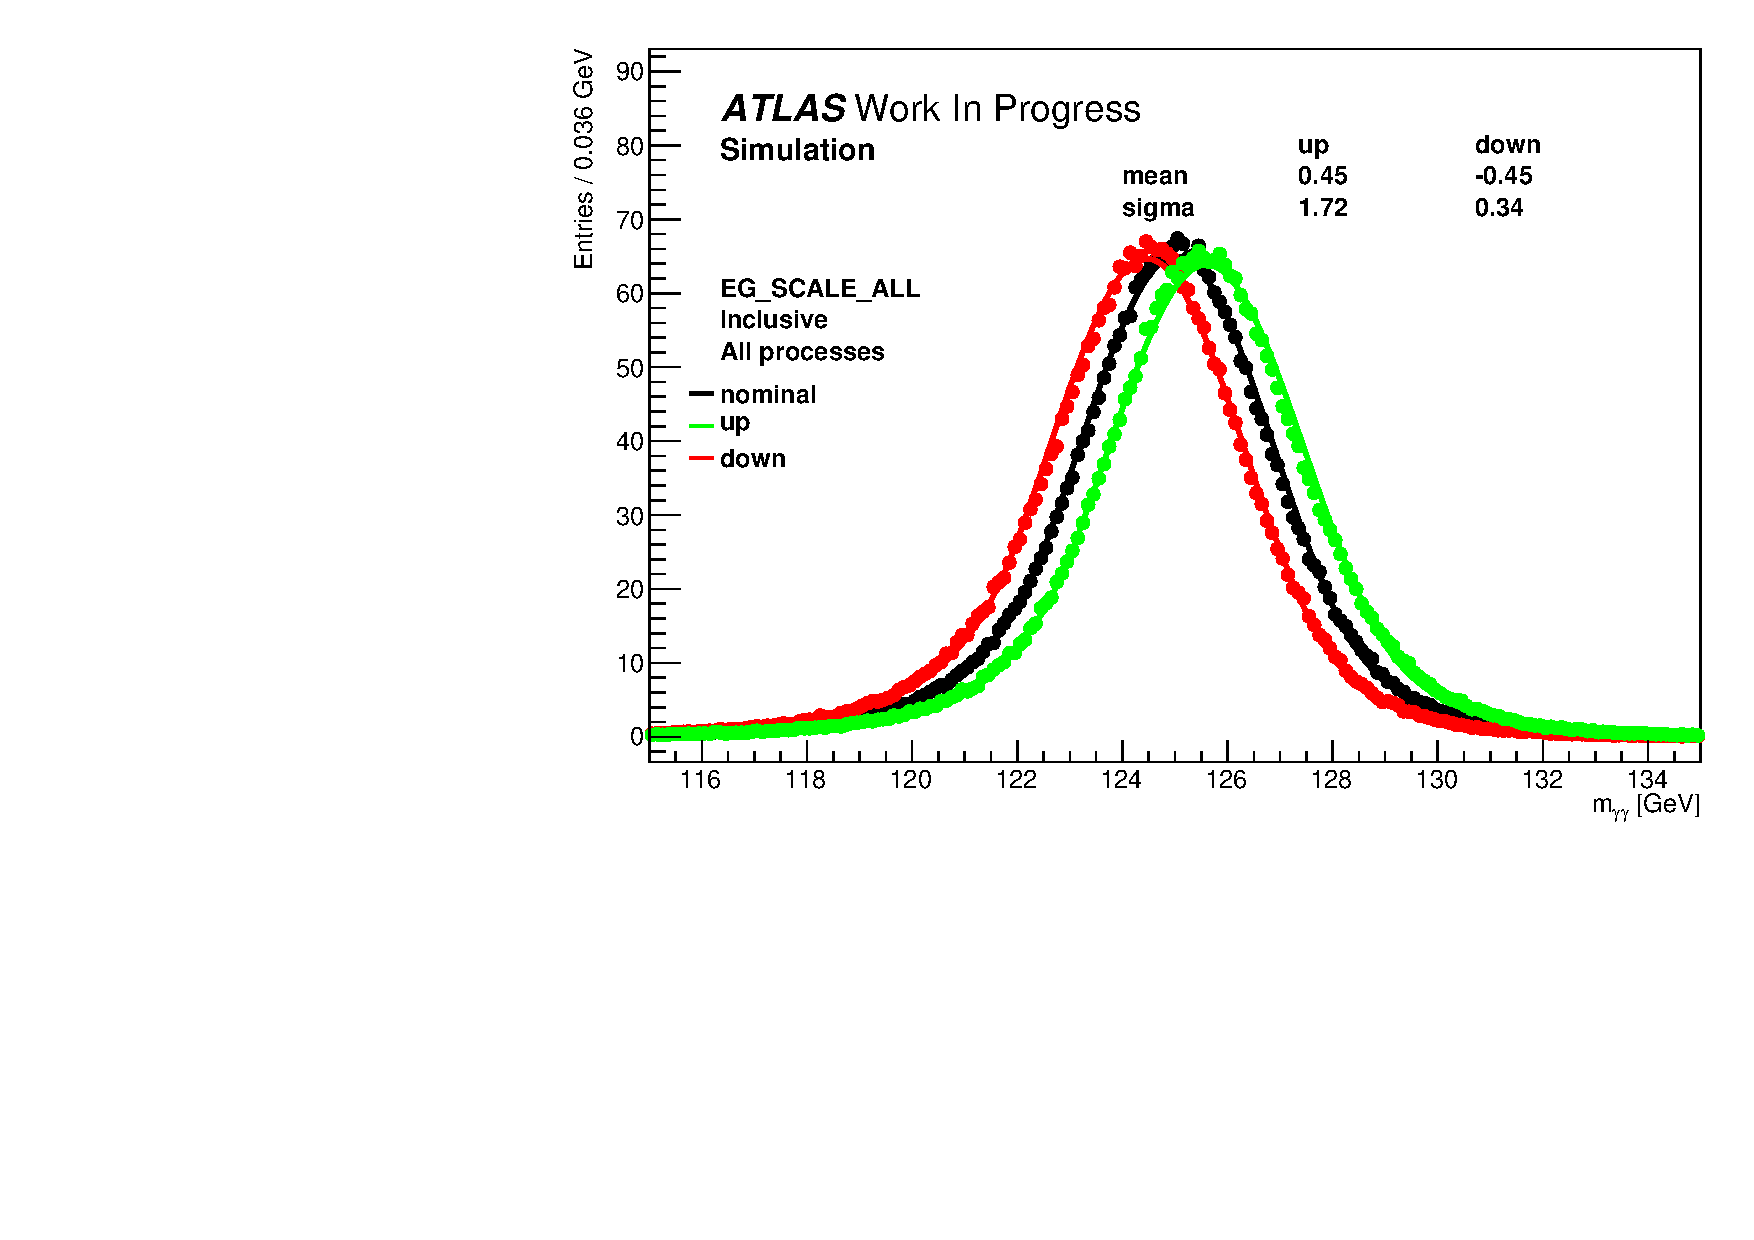
\includegraphics[width=.9\linewidth]{/home/goudet/Documents/LAL/Slides/Misc/plots/h015_ALL_root_SystVariation_EG_SCALE_ALL_0.pdf}
\end{center}
\end{column}
\end{columns}
\begin{columns}
\begin{column}{0.45\columnwidth}
\begin{center}
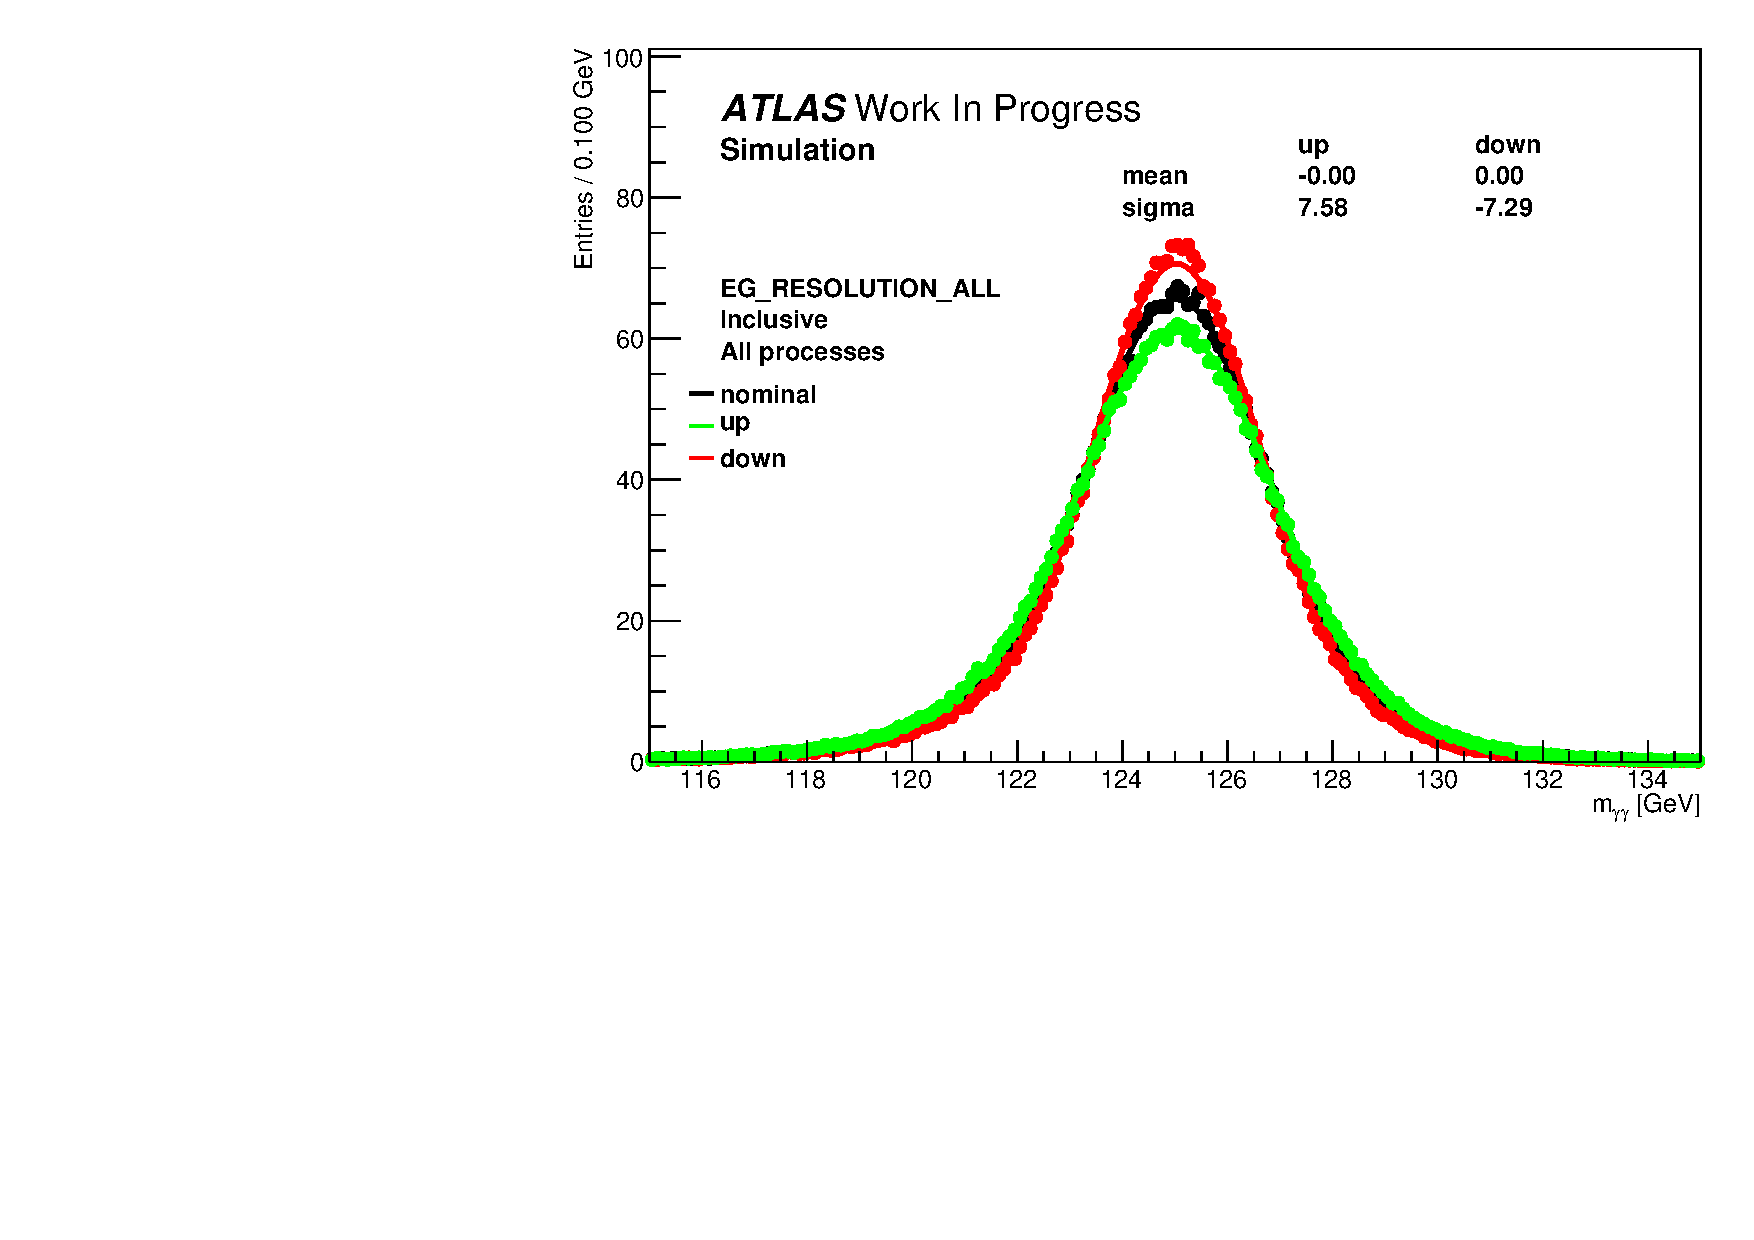
\includegraphics[width=.9\linewidth]{/home/goudet/Documents/LAL/Slides/Misc/plots/h015_ALL_SystVariation_EG_RESOLUTION_ALL_0.pdf}
\end{center}
\end{column}
\begin{column}{0.45\columnwidth}
\begin{center}
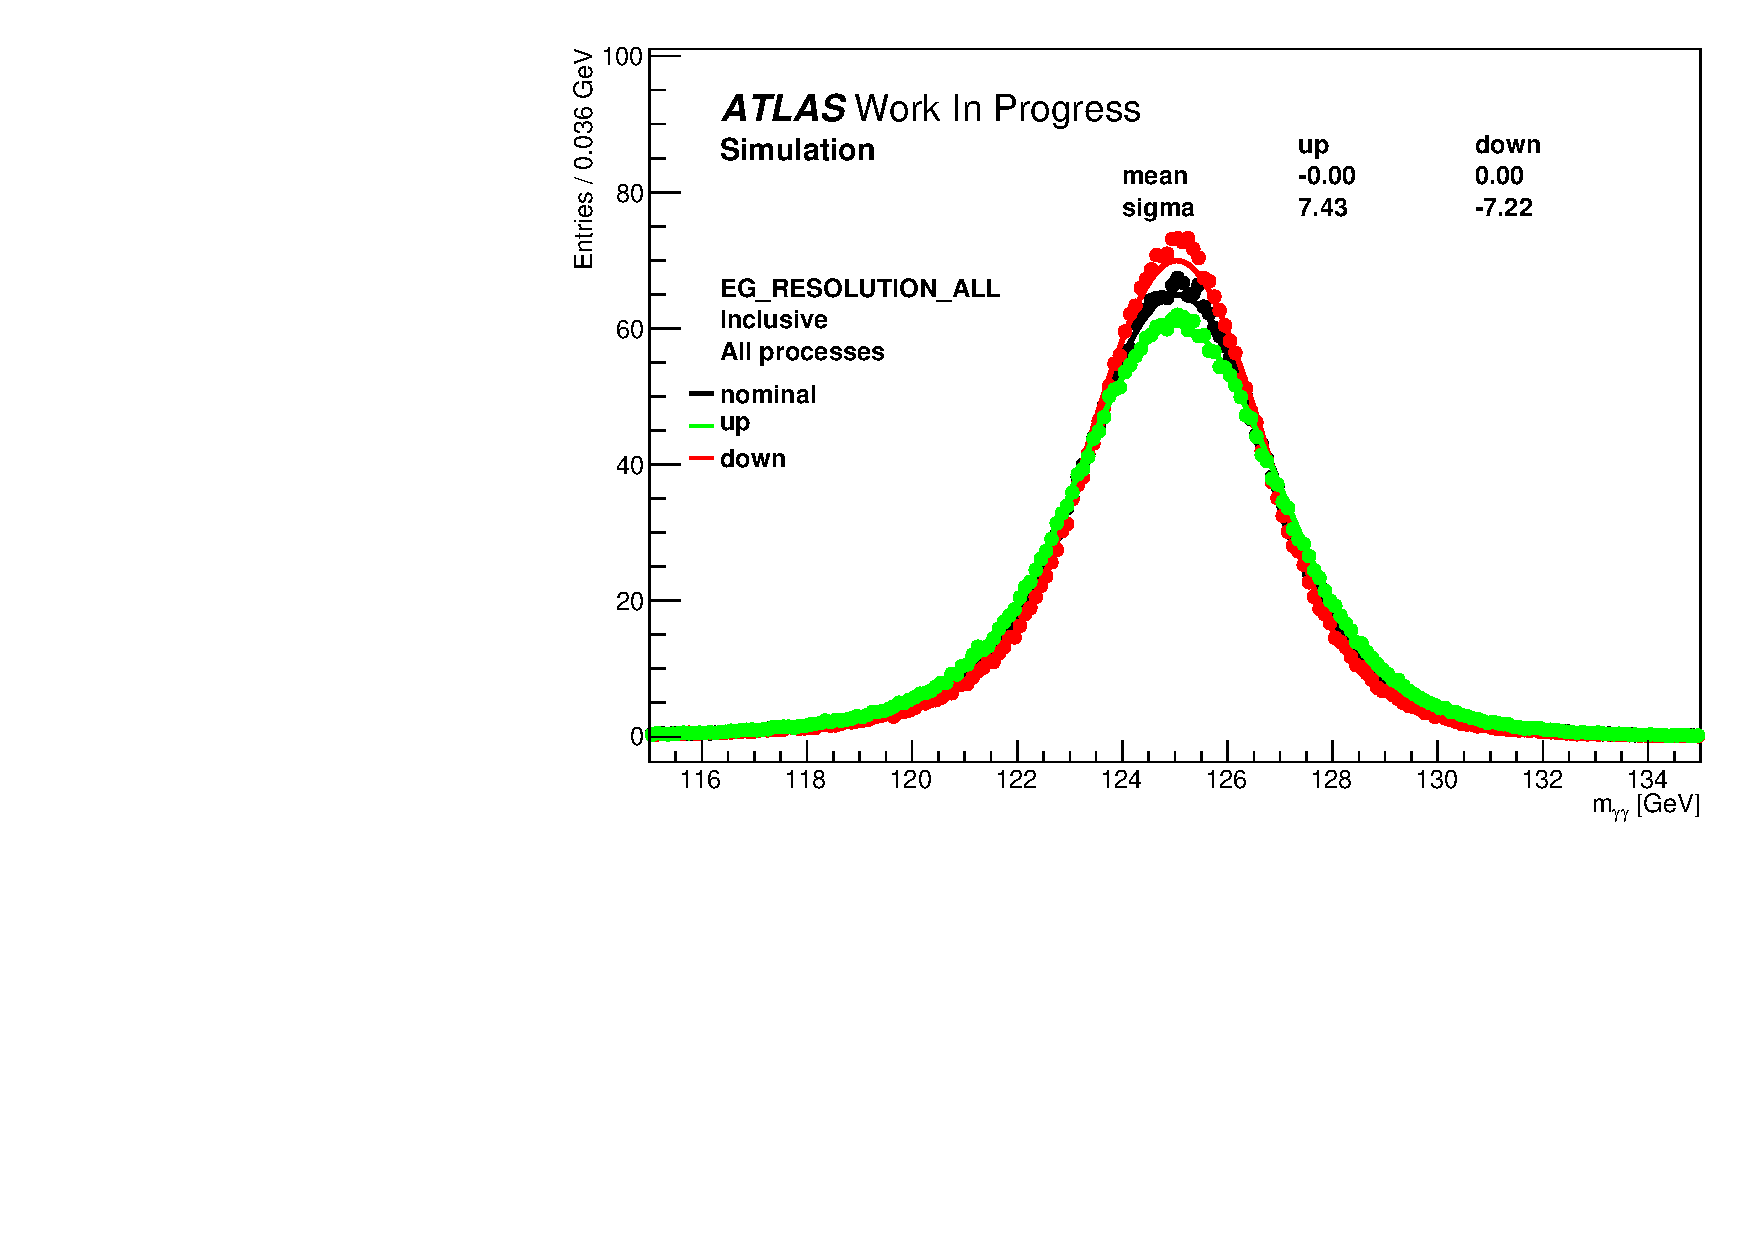
\includegraphics[width=.9\linewidth]{/home/goudet/Documents/LAL/Slides/Misc/plots/h015_ALL_root_SystVariation_EG_RESOLUTION_ALL_0.pdf}
\end{center}
\end{column}
\end{columns}
\end{frame}
\begin{frame}[label={sec:orgb38dd87}]{Categories}
ROOT and RooFit methods shows significant difference in VH and ttH categories
\begin{columns}
\begin{column}{0.5\columnwidth}
\begin{center}
\includegraphics[width=.9\linewidth]{/home/goudet/Documents/LAL/Zim/Hgam/PhotonSystematic/170309_CompareFits_h015_mean.pdf}
\end{center}
\end{column}



\begin{column}{0.5\columnwidth}
\begin{center}
\includegraphics[width=.9\linewidth]{/home/goudet/Documents/LAL/Zim/Hgam/PhotonSystematic/170309_CompareFits_h015_sigma.pdf}
\end{center}
\end{column}
\end{columns}
\end{frame}


\begin{frame}[label={sec:org4798c9c}]{RESOLUTION VHBSM}
\begin{center}
\tiny
\begin{tabular}{lrrrrrr}
\hline
NP & mean & sigma & alphaHi & alphaLow & nHi & nLow\\
\hline
\hline
RooFit &  &  &  &  &  & \\
\hline
Nominal & 125.144 & 0.120372 & 0.207774 & 0.1117 & 1.24293 & 13.9984\\
EG\(_{\text{RESOLUTION}}\)\(_{\text{ALL}}\)\_\(_{\text{1down}}\) & 125.338 & 0.111511 & 0.207774 & 0.1117 & 1.24293 & 13.9984\\
EG\(_{\text{RESOLUTION}}\)\(_{\text{ALL}}\)\_\(_{\text{1up}}\) & 125.053 & 0.129649 & 0.207774 & 0.1117 & 1.24293 & 13.9984\\
EG\(_{\text{SCALE}}\)\(_{\text{ALL}}\)\_\(_{\text{1down}}\) & 124.352 & 0.117578 & 0.207774 & 0.1117 & 1.24293 & 13.9984\\
EG\(_{\text{SCALE}}\)\(_{\text{ALL}}\)\_\(_{\text{1up}}\) & 125.941 & 0.12559 & 0.207774 & 0.1117 & 1.24293 & 13.9984\\
\hline
\hline
ROOT &  &  &  &  &  & \\
\hline
Nominal & 124.919 & 0.919806 & 0.487448 & 1.08326 & 6.73773 & 3.7769\\
EG\(_{\text{RESOLUTION}}\)\(_{\text{ALL}}\)\_\(_{\text{1down}}\) & 125.001 & 0.828496 & 0.487448 & 1.08326 & 6.73773 & 3.7769\\
EG\(_{\text{RESOLUTION}}\)\(_{\text{ALL}}\)\_\(_{\text{1up}}\) & 124.877 & 0.890828 & 0.487448 & 1.08326 & 6.73773 & 3.7769\\
EG\(_{\text{SCALE}}\)\(_{\text{ALL}}\)\_\(_{\text{1down}}\) & 124.211 & 0.955802 & 0.487448 & 1.08326 & 6.73773 & 3.7769\\
EG\(_{\text{SCALE}}\)\(_{\text{ALL}}\)\_\(_{\text{1up}}\) & 125.624 & 0.919994 & 0.487448 & 1.08326 & 6.73773 & 3.7769\\
\hline
\end{tabular}
\end{center}

\begin{columns}
\begin{column}{0.5\columnwidth}
\begin{center}
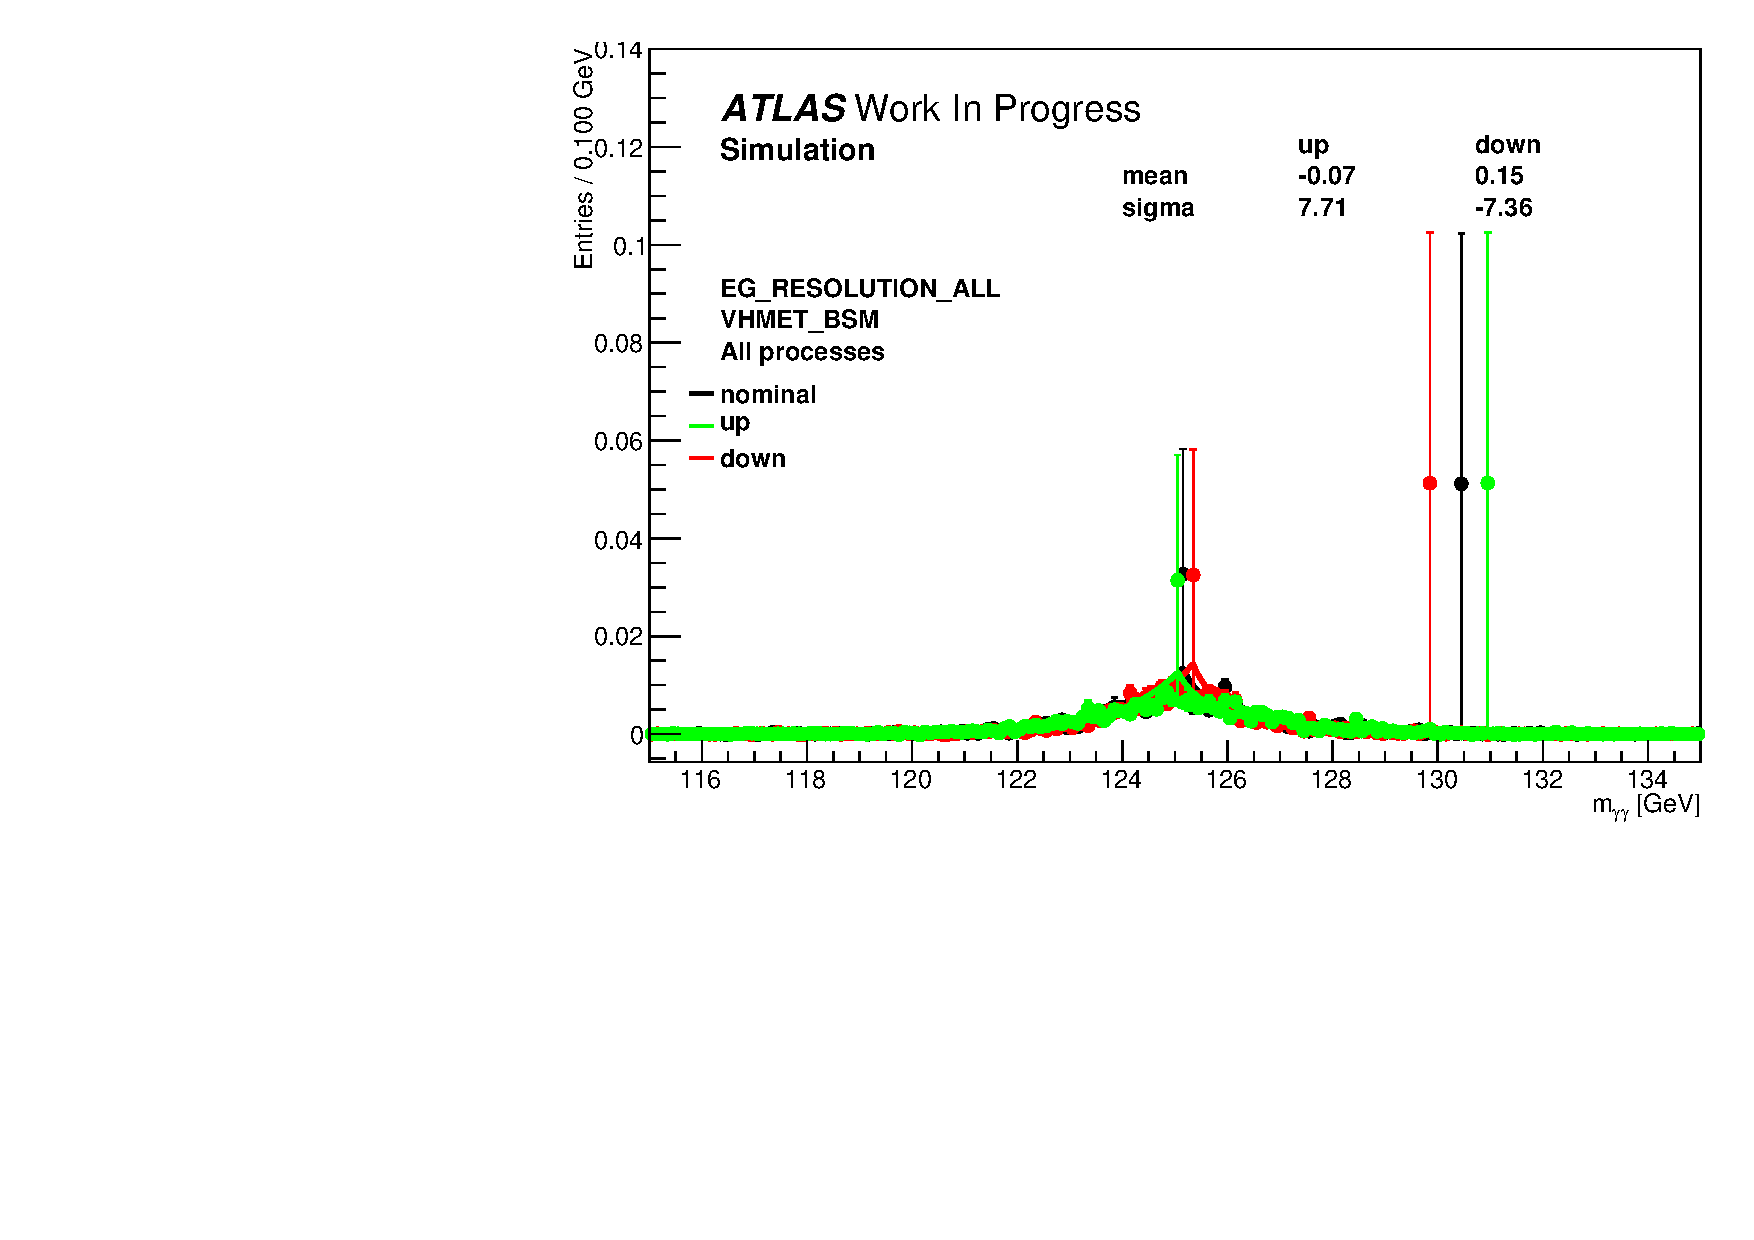
\includegraphics[width=.9\linewidth]{/home/goudet/Documents/LAL/Slides/Misc/plots/h015_ALL_SystVariation_EG_RESOLUTION_ALL_20.pdf}
\end{center}
\end{column}

\begin{column}{0.5\columnwidth}
\begin{center}
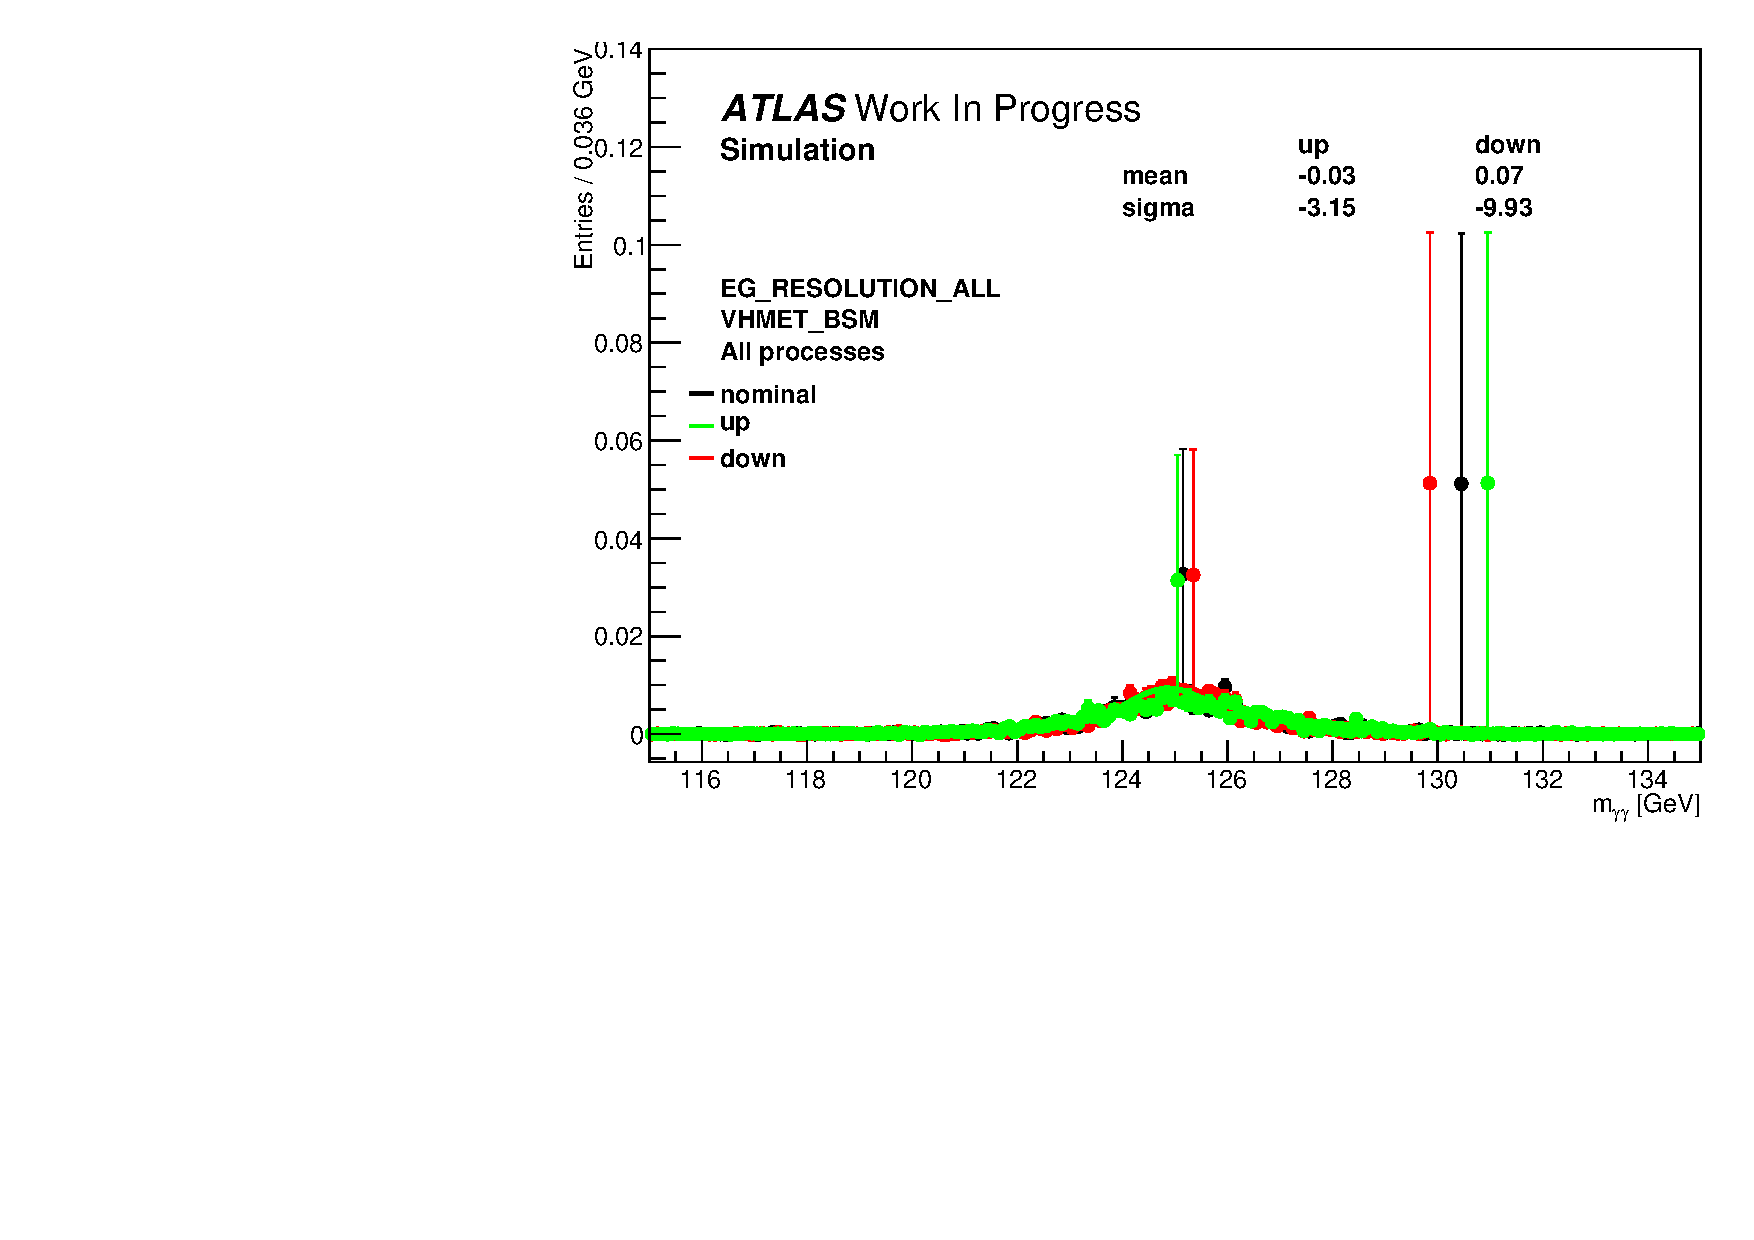
\includegraphics[width=.9\linewidth]{/home/goudet/Documents/LAL/Slides/Misc/plots/h015_ALL_root_SystVariation_EG_RESOLUTION_ALL_20.pdf}
\end{center}
\end{column}
\end{columns}
\end{frame}
\end{document}